\documentclass[journal]{IEEEtran}

\usepackage[spanish]{babel}
\usepackage[utf8]{inputenc}
\usepackage[T1]{fontenc}
\usepackage{graphicx}
\usepackage{amssymb}
\usepackage{amsmath}
\usepackage{amsthm}
\usepackage{booktabs}
\usepackage{gensymb}
\usepackage{stfloats}
\usepackage{float}
\usepackage{nccmath}
\usepackage{caption}
\usepackage{url}

\title{\textbf{Packet Tracer y eNSP}}

\author{Redes LAN y WAN \\
	\textit{Docentes:} Luis Fernando Díaz Cadavid - Jaime Alberto Sepúlveda\\ 
	\textit{Monitores:} Juan José Jaramillo Granada \\
	Kevin Leonardo Cerpa Campanella \\
	Universidad Nacional de Colombia - Sede Manizales}

\date{}

\begin{document}
\maketitle

\section{Descripción}
\textbf{\textit{Cisco Packet Tracer}} es un simulador de redes de telecomunicaciones que nos permite realizar diseños de topologías, configurar los dispositivos de red, detectar y corregir errores en redes de una manera casi idéntica a la realidad. Una ventaja adicional es que nos permite analizar cada proceso que se ejecuta en la simulación de acuerdo a la capa de modelo OSI que interviene en dicho proceso. La limitación actual de este software es que propone un monopolio con los modelos CISCO, ya que hoy en día compañías como Huawei están lanzando diversos tipos de dispotivos para lo cual debemos utilizar otro emulador de redes. Se encuentra disponible en los sistemas operativos Linux, Android 4.1+, iOS 8+ y Microsoft Windows \cite{pt_wiki} \newline
\textbf{\textit{eNSP}} al igual que Packet Tracer es un simulador de redes de datos cuyo propietario es Huawei Technologies en el cual se promueve sus modelos e interfaces de una manera más libre.

\section{El Entorno de Packet Tracer}
Al instalar Cisco Packet Tracer 7.2.1 nos pedirá que nos registremos en el portal de CISCO para poder permitir el ingreso al software, luego de ingresar al software veremos la siguiente interfaz:

\begin{figure}[ht]
	\centering
	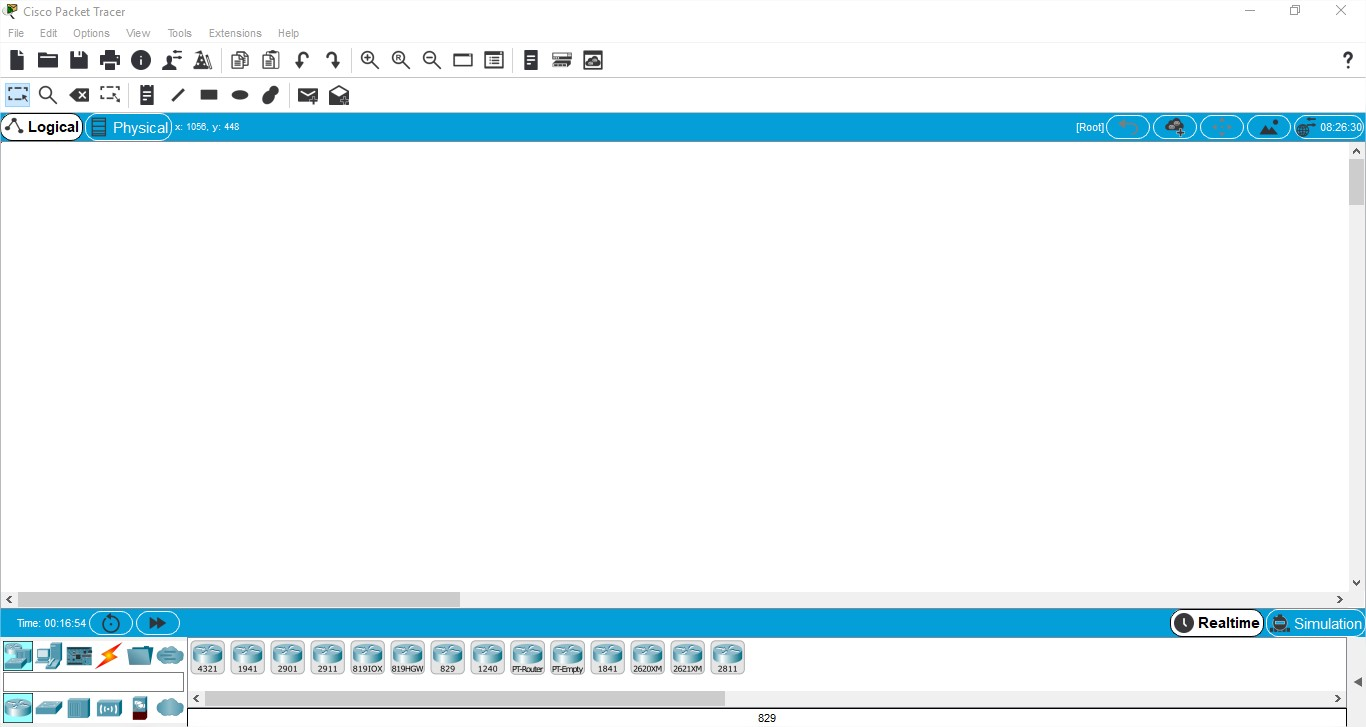
\includegraphics[scale=0.17]{index_pt.jpg}
	\caption{Interfaz de inicio Packet Tracer}
	\label{index_pt}
\end{figure}

Packet Tracer presenta tres modos de operación, el primero de estos es el modo de topología, que es el de la imagen anterior la cual muestra la pantalla de inicio del programa, el segundo modo es el de simulación el cual se accede al correr el modelo de red creado en el modo de topología, y el tercer modo es un modo en tiempo real, en donde se pueden programar mensajes para detectar dispositivos que están activos en la red y permite detectar problemas de direccionamiento o tamaño de tramas entre las conexiones.

\subsection{Modo de Topología}
En este modo se realizan tres tareas principales, la primera de ellas es el diseño de la red mediante la creación y organización de dispositivos; por consiguiente en este modo de operación se dispone de:
\begin{enumerate}
	\item Menú de operaciones del proyecto.
		\begin{figure}[ht]
			\centering
			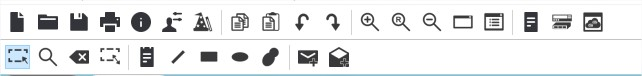
\includegraphics[scale=0.4]{pt_menuoperaciones.jpg}
			\caption{Menú de operaciones de Packet Tracer}
		\end{figure}
	\item Área de trabajo.
		\begin{figure}[ht]
			\centering
			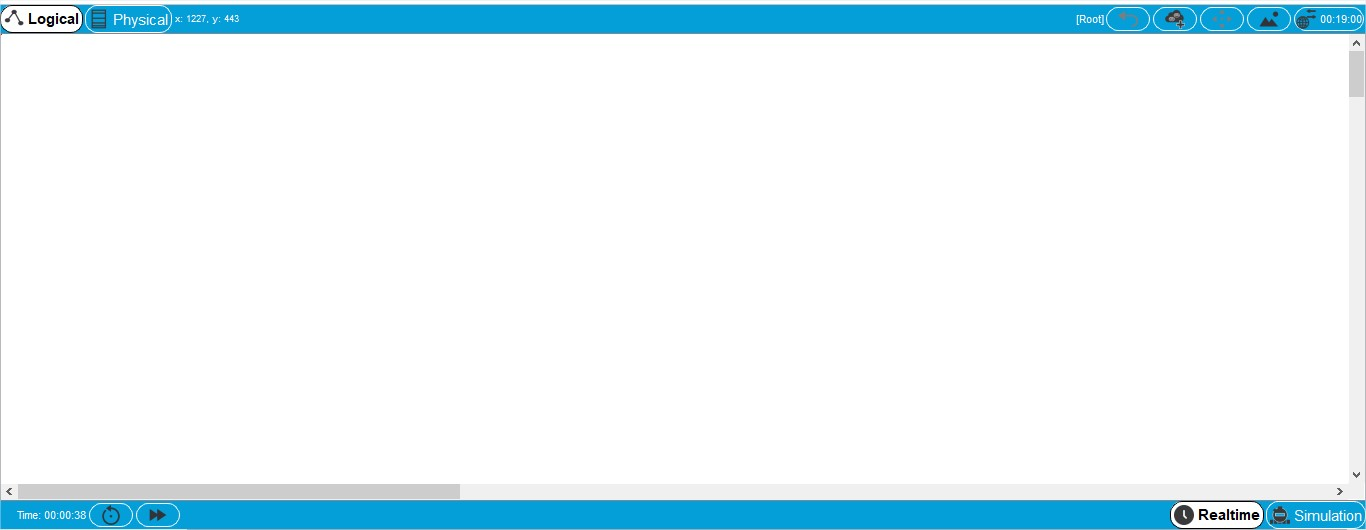
\includegraphics[scale=0.19]{pt_areatrabajo.jpg}
			\caption{Área de trabajo de Packet Tracer}
		\end{figure}
	\item Panel de dispositivos disponibles
		\begin{figure}[ht]
			\centering
			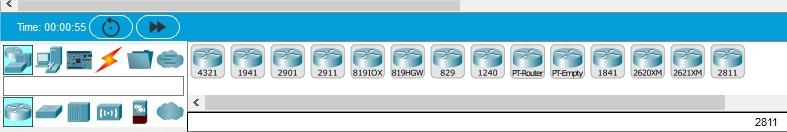
\includegraphics[scale=0.44]{pt_paneldispositivos.jpg}
			\caption{Panel de dispositivos de Packet Tracer}
		\end{figure}
\end{enumerate}

\subsection{Simulación}
Se programan los paquetes que se van a transmitir por la red que previamente se ha modelado. Dentro de este modo de operación se visualiza el proceso de transmisión y recepción de información.
\begin{figure}[ht]
	\centering
	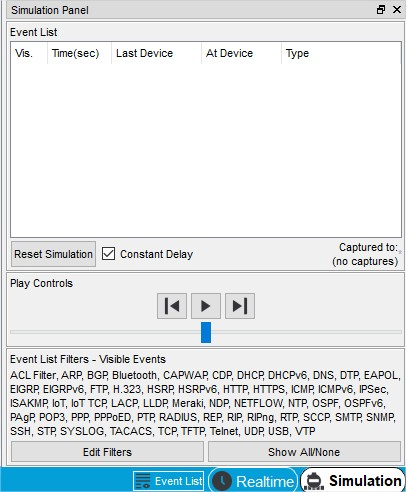
\includegraphics[scale=0.3]{pt_simulation.jpg}
	\caption{Modo de simulaciòn de Packet Tracer}
\end{figure}

\newpage

\subsection{Realtime}
Esta diseñado para enviar comandos de prueba con el objetivo de reconocer los dispositivos de la red que están activos, y comprobar que se pueden transmitir paquetes de un servidor a otro en la red. 

\begin{figure}[ht]
	\centering
	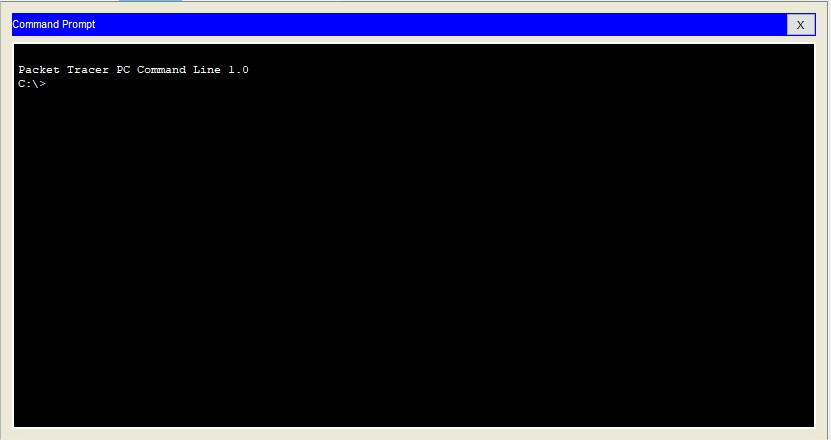
\includegraphics[scale=0.3]{pt_realtime.jpg}
	\caption{Modo en tiempo real de los dispositivos de Packet Tracer}
\end{figure}

\section{Red LAN Básica en Packet Tracer}

\subsection{Implementación}
Ahora realizaremos una red LAN básica, donde podamos comprobar tanto en cada modo de operación de packet tracer el correcto funcionamiento de esta.
\newline
Se propone realizar una red LAN entre tres computadoras, para esto se necesita un Switche como dispositivo de interconexión entre ellos. \\
Para ello se toma del panel de dispositivos en la pestaña de \textit{Network Devices} un \textit{PT-Switch}:

\begin{figure}[ht]
	\centering
	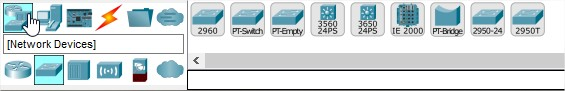
\includegraphics[scale=0.4]{pt_switch.jpg}
\end{figure}

\newpage

Luego se toman de la pestaña \textit{End Devices} tres \textit{PC} y se arrastran al área de trabajo:

\begin{figure}[ht]
	\centering
	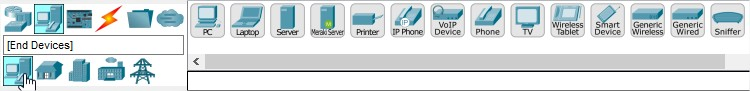
\includegraphics[scale=0.37]{pt_devices.jpg}
\end{figure}

Por defecto cada dispositivo en la red se va a encontrar encendido y cada elemento PC viene con un puerto Ethernet incorporado, que para conectarlo al Switch seleccionamos el conector de la sección \textit{Connections} que se muestra a continuación:

\begin{figure}[ht]
	\centering
	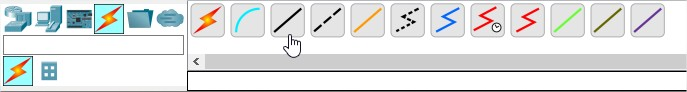
\includegraphics[scale=0.4]{pt_connections.jpg}
\end{figure}

Luego de seleccionar la conexión ponemos el puntero del mouse sobre el elemento a conectar y nos mostrará los puertos disponibles así:

\begin{figure}[ht]
	\centering
	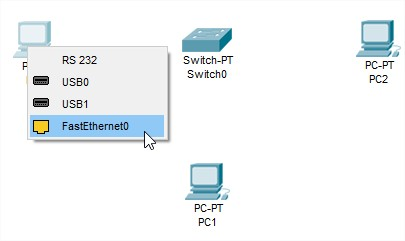
\includegraphics[scale=0.5]{pt_connectionpc.jpg}
\end{figure}

Luego de hacer conexión nos mostrará el cable cuyo otro extremo necesita ser conectado, y nos vamos al Switche y realizamos el mismo procedimiento así:

\begin{figure}[ht]
	\centering
	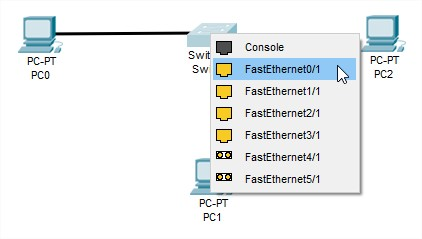
\includegraphics[scale=0.5]{pt_connectionswitch.jpg}
\end{figure}

Y realizamos el mismo procedimiento para el resto de computadoras de la red.
\newline \newline
Por último nos vamos a la configuración de cada pc en su red y les asignamos diferentes direcciones IP privadas a cada pc.

\newpage

Para ello nos vamos a las propiedades de cada pc, luego a la pestaña desktop y luego a ip configuration:

\begin{figure}[ht]
	\centering
	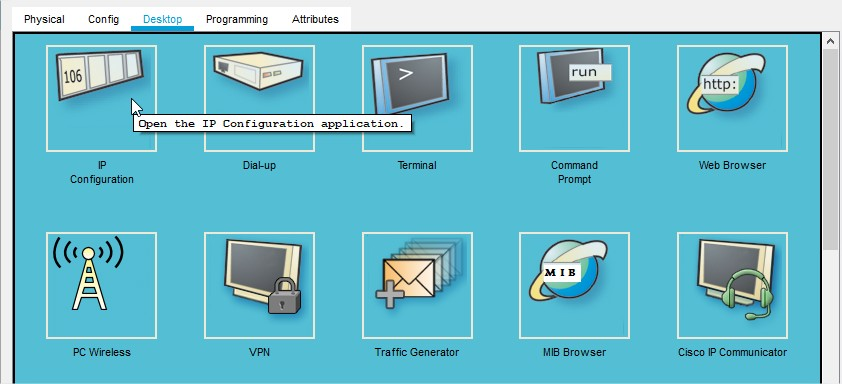
\includegraphics[scale=0.3]{pt_menuip.jpg}
\end{figure}

Allí seleccionamos la opción \textit{Static} y agregamos diferente dirección IP Clase B a cada dispositivo y la misma máscara de subred (dirección IP Clase C).

\begin{figure}[ht]
	\centering
	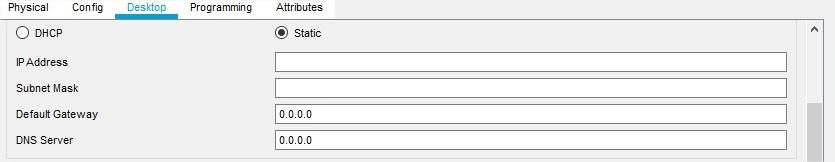
\includegraphics[scale=0.5]{pt_ip.jpg}
\end{figure}

\subsection{Verificación}
Para verificar el correcto funcionamiento de la red debemos de comprobar que las señales o mensajes que se envien de un computador a otro lleguen correctamente. \\
Comprobaremos en cada modo de operación el correcto funcionamiento de la red como lo veremos en las siguientes secciones.
	\subsubsection{Verificación en Modo de Implementación}
	Observando el área de trabajo podremos ver que los extremos de las conexiones están con un triángulo verde:
	\begin{figure}[ht]
		\centering
		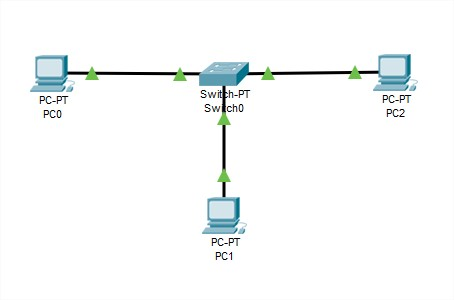
\includegraphics[scale=0.5]{pt_ver_modoimplementacion.jpg}
	\end{figure}	
	Esto indica que hay correcta comunicación, esto es una seña de que puede que la conexión este bien pero aún así no es suficiente, por ello debemos acudir a los demás modos de Packet Tracer
	\subsubsection{Verificación en Modo de Simulación}
	Para comprobar en este modo primeramente nos vamos al menù de operaciones en su parte inferior y seleccionamos el siguiente ícono:
	\begin{figure}[ht]
		\centering
		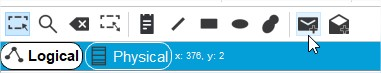
\includegraphics[scale=0.5]{pt_mensaje.jpg}
	\end{figure}
	Esto es para poder enviar un mensaje de un dispositivo a otro, así podremos verificar que hay una correcta conexión, para ellos luego de dar click como lo muestra la imagen anterior damos click en los dispositivos que queremos comprobar la conexión. \newline
	
	Luego de esto nos vamos al modo de simulación que se encuentra en la esquina inferior derecha del área de trabajo y damos en \textit{Simulation} y oprimimos en correr y se nos mostrará animadamente como el mensaje se envia de los dispositivos que seleccinoamos, así:
	\begin{figure}[ht]
		\centering
		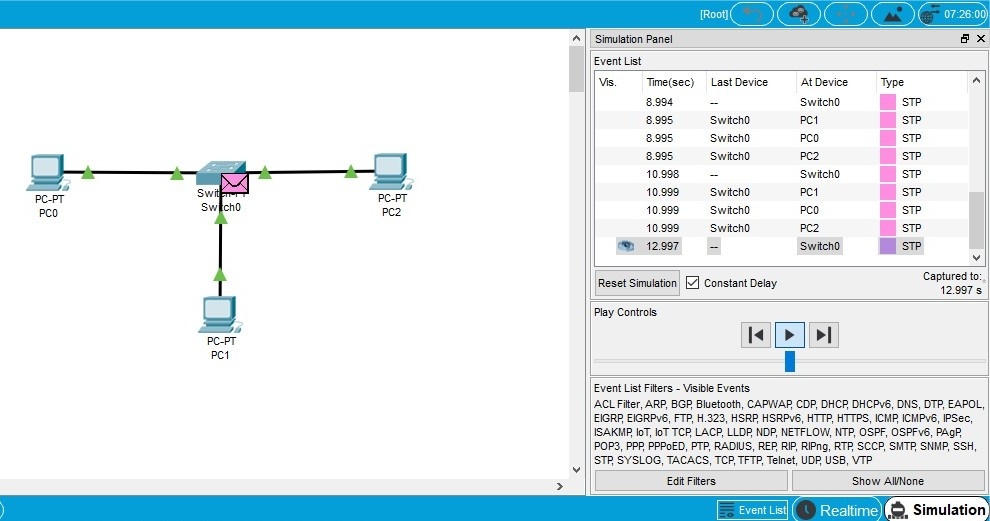
\includegraphics[scale=0.35]{pt_ver_simulation.jpg}
	\end{figure}
	
	\subsubsection{Verificación en Modo Realtime}
	Para verificar en modo realtime debemos entrar a la consola de comando de algún PC de la red implementada, esto lo hacemos entrando a las propiedades de éste (ya sea dando doble clik, o click secundario y \textit{Settings}), luego nos vamos a la pestaña Desktop y luego en la opción \textit{Command Prompt}, así: \newline
	\begin{figure}[ht]
		\centering
		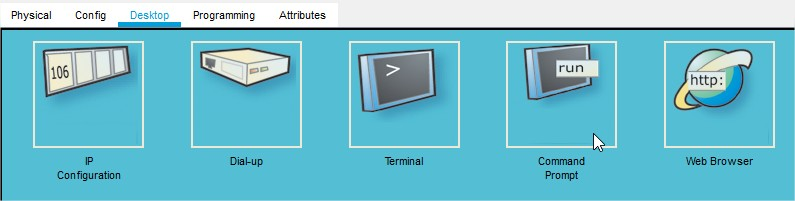
\includegraphics[scale=0.33]{pt_ver_realtime.jpg}
	\end{figure}

	\newpage

	Allí veremos el área realtime mostrada en la sección anterior y escribimos \textit{ping 'Dirección\_IP'} y la dirección IP privada de todos los elementos de la red, así:\newline
	\begin{figure}[ht]
		\centering
		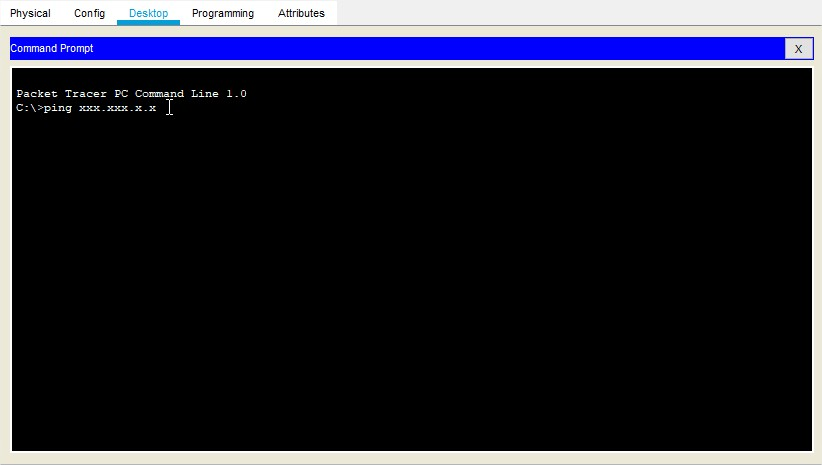
\includegraphics[scale=0.27]{pt_ver_ping1.jpg}
	\end{figure}
	
	Si la conexión está realizada correctamente debemos observar algo como lo siguiente:
	\begin{figure}[ht]
		\centering
		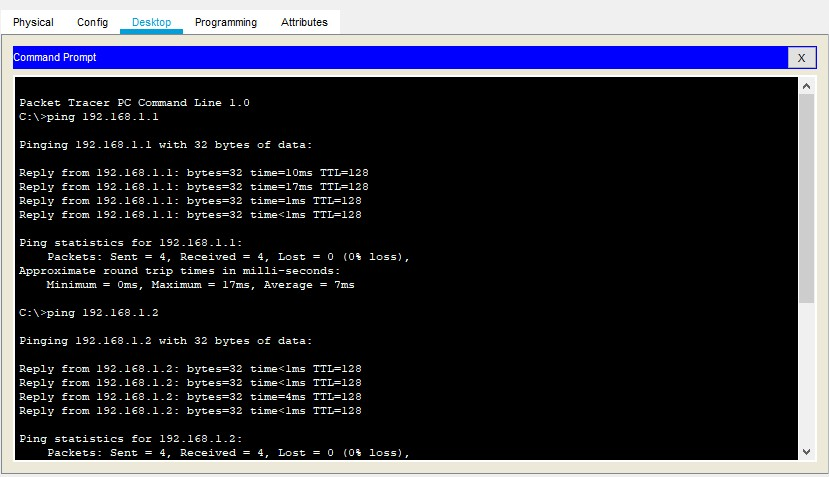
\includegraphics[scale=0.27]{pt_ver_ping2.jpg}
	\end{figure}
\section{EL ENTORNO DE eNSP}
Al ejecutar el software la primera imagen que obtendremos será la figura X en la que encontraremos algunos ejemplos bases que vienen con el programa y documentos introductorios para leer.
%%%%%%%%%%%%%%%
\begin{center}
\begin{figure}[H]
\centering
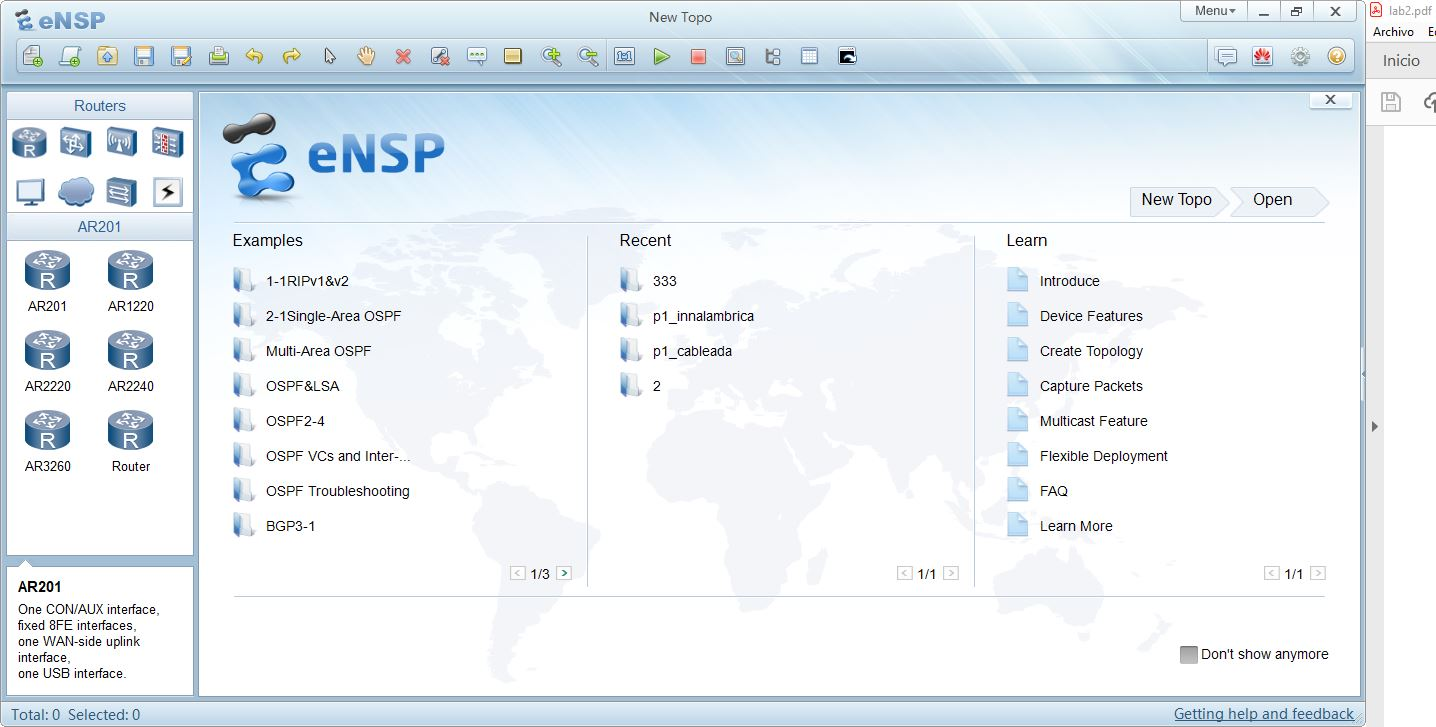
\includegraphics[scale=0.2]{0.JPG} 
\caption{Interfaz de inicio eNSP}
\end{figure}
\end{center}
%%%%%%%%%%%
En la esquina superior izquierda de la figura x encontraremos un botón (New Topo) que nos permitirá ingresar al área de trabajo.
%%%%%%%%%%%%%%%
\begin{center}
\begin{figure}[H]
\centering
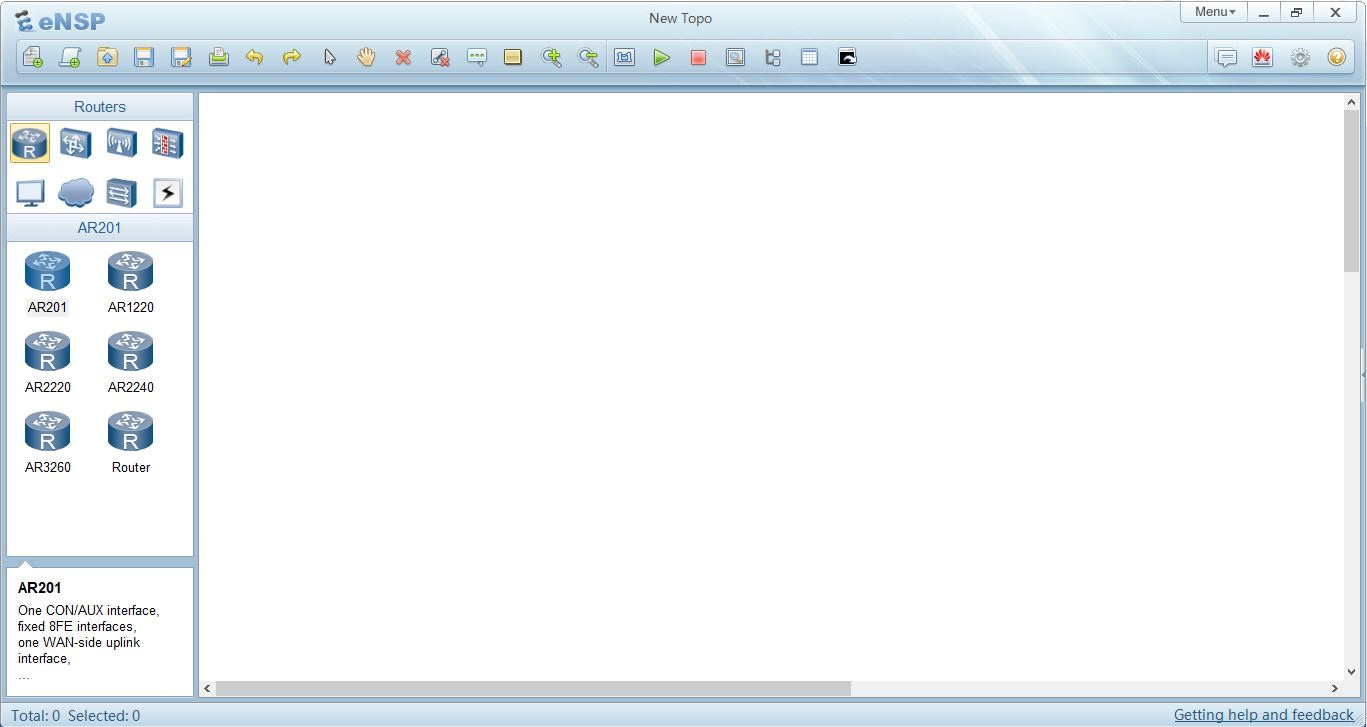
\includegraphics[scale=0.23]{1.JPG} 
\caption{Área de trabajo eNSP}
\end{figure}
\end{center}
%%%%%%%%%%%
A mano izquierda encontraremos nuestro Panel de dispositivos en el que encontraremos, routers, switches, WLAN, FireWall, end devices, other devices y conenections.
%%%%%%%%%%%%%%%
\begin{center}
\begin{figure}[H]
\centering
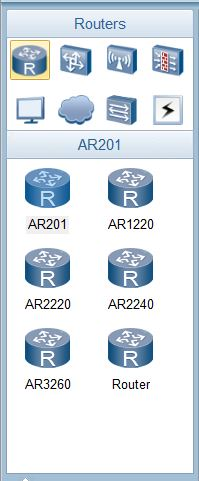
\includegraphics[scale=0.75]{2.JPG} 
\caption{Panel de dispositivos de eNSP}
\end{figure}
\end{center}
%%%%%%%%%%%
\section{RED LAN BÁSICA EN eNSP}
\subsection{Implementación}
Desarrollaremos la misma red LAN que se realizó en el Packet Tracer utilizando ahora el simulador de Huawei.\\
Para ello se toma del panel de dispositivos en la pestaña de \textit{Switches} un S5700 y se arrastra a el área de trabajo.
\begin{center}
\begin{figure}[H]
\centering
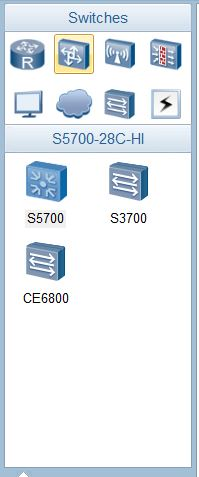
\includegraphics[scale=0.65]{3.JPG} 
\end{figure}
\end{center}
%%%%%%%%%%%
De igual forma se toman de la pestaña \textit{End Devices} tres PC y se arrastran.
\begin{center}
\begin{figure}[H]
\centering
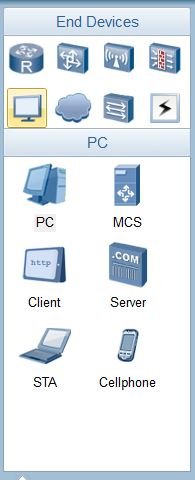
\includegraphics[scale=0.65]{4.JPG} 
\end{figure}
\end{center}
%%%%%%%%%%%
Por defecto cada dispositivo en la red se va a encontrar encendido y cada elemento PC viene con un puerto Ethernet incorporado, que para conectarlo al Switch seleccionamos el conector cooper en la seccion Connections que se muestra a continuación:
%%%%%%%%%%%%%%%
\begin{center}
\begin{figure}[H]
\centering
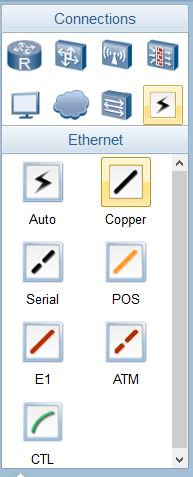
\includegraphics[scale=0.65]{5.JPG} 
\end{figure}
\end{center}
%%%%%%%%%%%
Luego de seleccionar la conexión ponemos el puntero del mouse sobre el elemento a conectar y nos mostrará los puertos disponibles así:
%%%%%%%%%%%%%%%
\begin{center}
\begin{figure}[H]
\centering
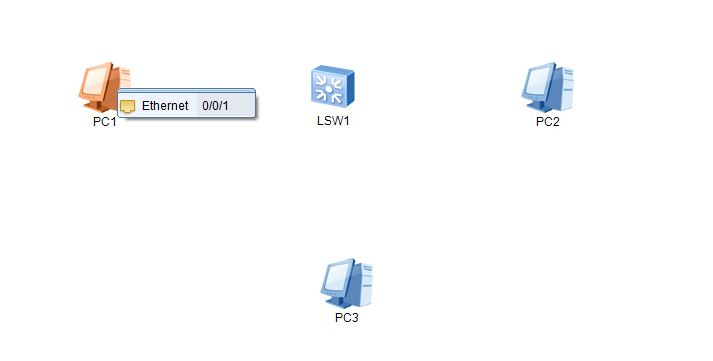
\includegraphics[scale=0.5]{6.JPG} 
\end{figure}
\end{center}
%%%%%%%%%%%
Luego de hacer conexión nos mostrará el cable cuyo otro extremo necesita ser conectado, y nos vamos al Switche y realizamos el mismo procedimiento así:
%%%%%%%%%%%%%%%
\begin{center}
\begin{figure}[H]
\centering
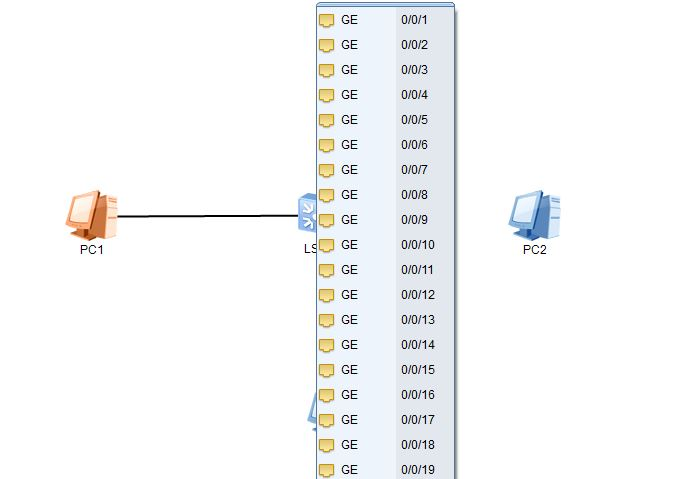
\includegraphics[scale=0.5]{7.JPG} 
\end{figure}
\end{center}
%%%%%%%%%%%
Y realizamos el mismo procedimiento para el resto de computadoras de la red.
Por último nos vamos a la configuración de cada pc en su red y les asignamos diferentes direcciones IP privadas y su respectiva  mascara de red a cada pc.\\
 
Para ellos cliqueamos cada dispositivo una vez con el click derecho en el que encontraremos lo siguiente:
%%%%%%%%%%%%%%%
\begin{center}
\begin{figure}[H]
\centering
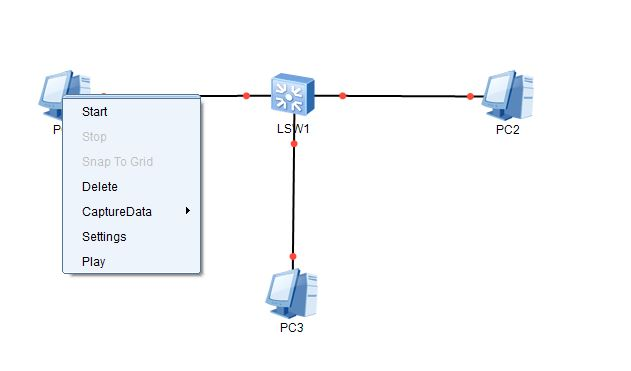
\includegraphics[scale=0.5]{8.JPG} 
\end{figure}
\end{center}
%%%%%%%%%%%
Entramos a configuración donde nos espera una ventana, alli seleccionamos la opción Static y agregamos diferente dirección IP Clase B a cada dispositivo y la misma máscara de subred (dirección IP Clase C).
%%%%%%%%%%%%%%%
\begin{center}
\begin{figure}[H]
\centering
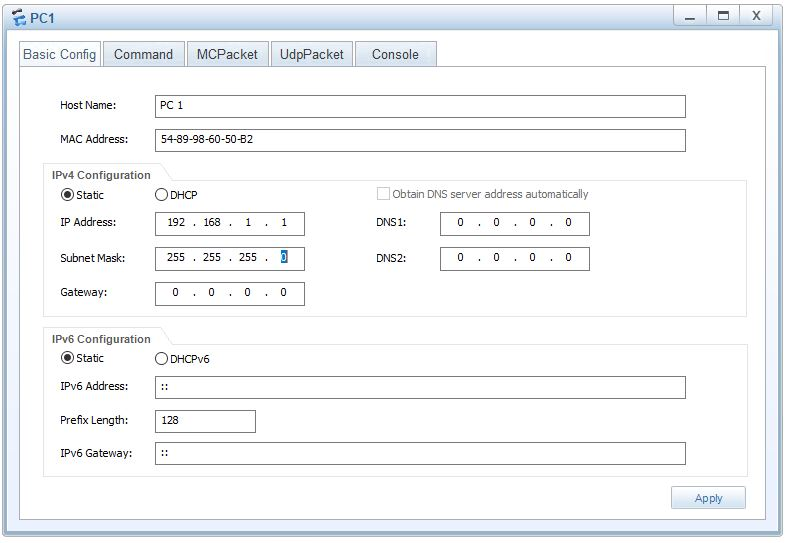
\includegraphics[scale=0.42]{9.JPG} 
\end{figure}
\end{center}
%%%%%%%%%%%
\subsection{Verificación:}
Para verificar el correcto funcionamiento de la red debemos de comprobar que las señales o mensajes que se envíen de un computador a otro lleguen correctamente.\\
Para esto lo primero que tenemos que hacer es seleccionar todos los dispositivos e iniciarlos, los puntos de conexión  se pondrán de color verde.
%%%%%%%%%%%%%%%
\begin{center}
\begin{figure}[H]
\centering
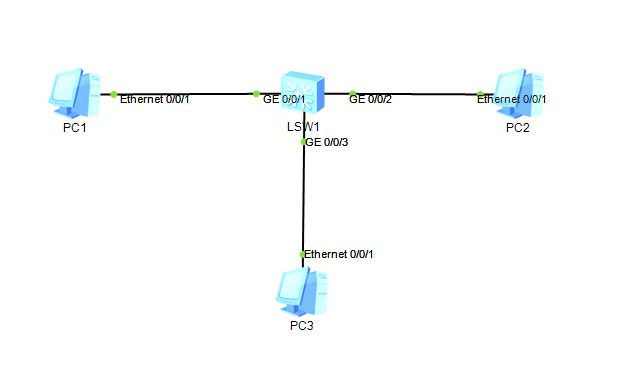
\includegraphics[scale=0.55]{10.JPG} 
\end{figure}
\end{center}
%%%%%%%%%%%
Esto indica que hay correcta comunicación, esto es una seña de que puede que la conexión este bien pero aun así no es suficiente, por lo que acudiremos a una herramientas del eNSP.\\
\subsubsection{Wireshark}
Wireshark, antes conocido como Ethereal, es un analizador de protocolos utilizado para realizar análisis y solucionar problemas en redes de comunicaciones, para desarrollo de software y protocolos, y como una herramienta didáctica.\\
Para ingresar a esta herramienta seleccionamos el dispositivo, cliqueamos para ver las opciones y nos dirigimos a captura de datos donde debemos hacer click en la conexión que queremos comprobar.
%%%%%%%%%%%%%%%
\begin{center}
\begin{figure}[H]
\centering
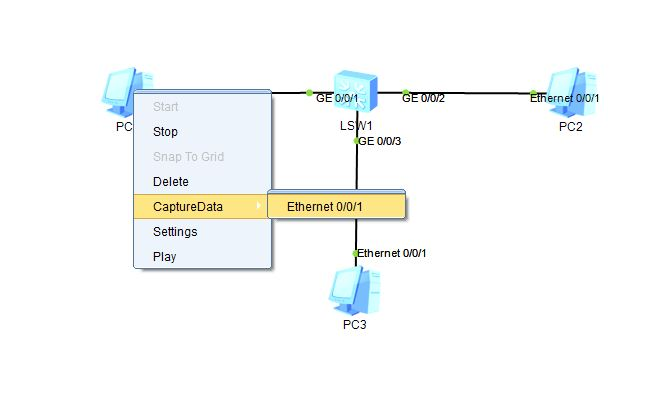
\includegraphics[scale=0.55]{11.JPG} 
\end{figure}
\end{center}
%%%%%%%%%%%
A continuación se nos abrirá la ventana: 
%%%%%%%%%%%%%%%
\begin{center}
\begin{figure}[H]
\centering
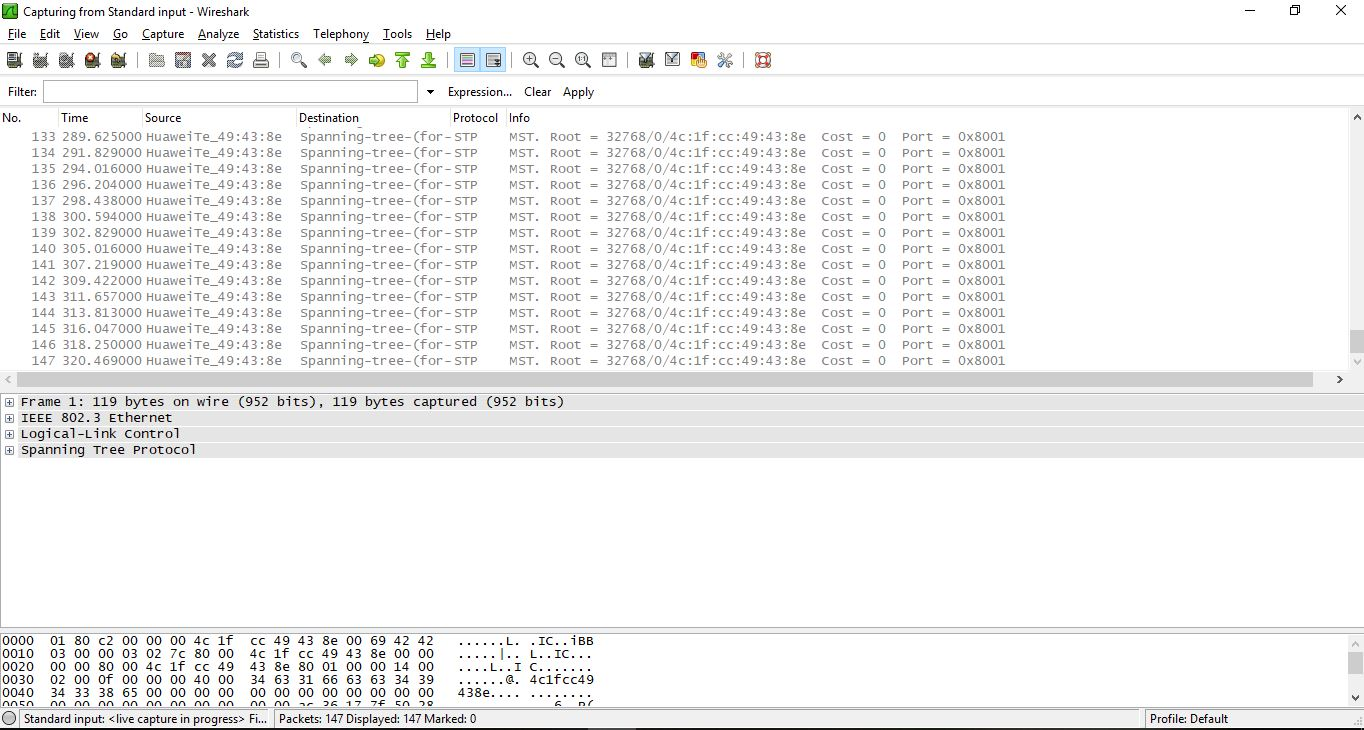
\includegraphics[scale=0.25]{13,5.JPG} 
\end{figure}
\end{center}
%%%%%%%%%%%
Procedemos a generar un ping de prueba ingresando al Cmd del PC 1, el cual se encuentra en una de las pestañas de la ventana de configuración.
%%%%%%%%%%%%%%%
\begin{center}
\begin{figure}[H]
\centering
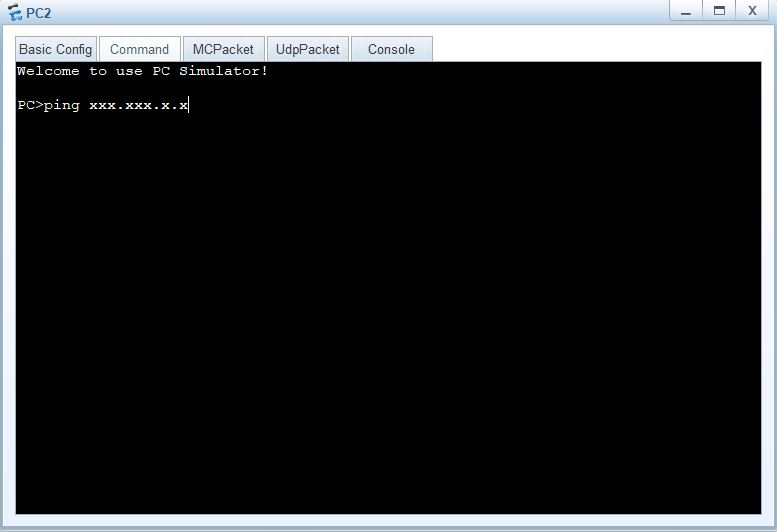
\includegraphics[scale=0.4]{12,5.JPG} 
\end{figure}
\end{center}
%%%%%%%%%%%
Si la conexión está realizada correctamente debemos observar algo como lo siguiente:
%%%%%%%%%%%%%%%
\begin{center}
\begin{figure}[H]
\centering
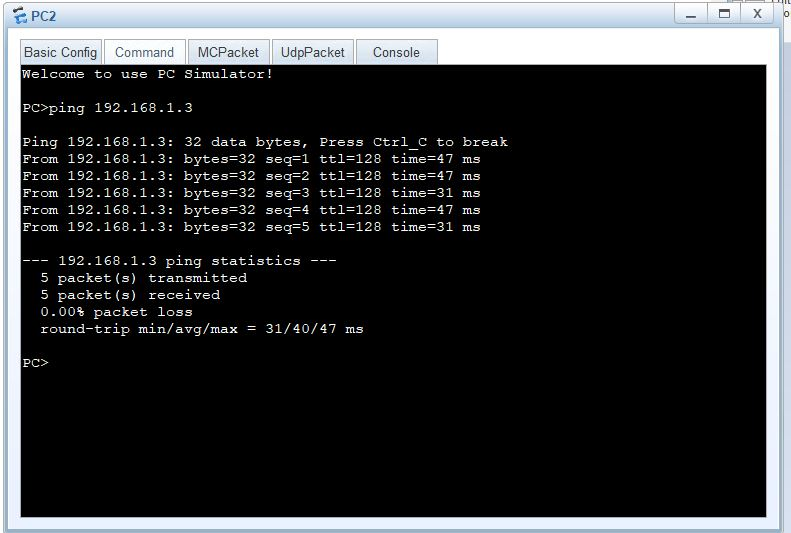
\includegraphics[scale=0.4]{12.JPG} 
\end{figure}
\end{center}
%%%%%%%%%%%
Y en el  Wireshark. Deberíamos observar:
%%%%%%%%%%%%%%%
\begin{center}
\begin{figure}[H]
\centering
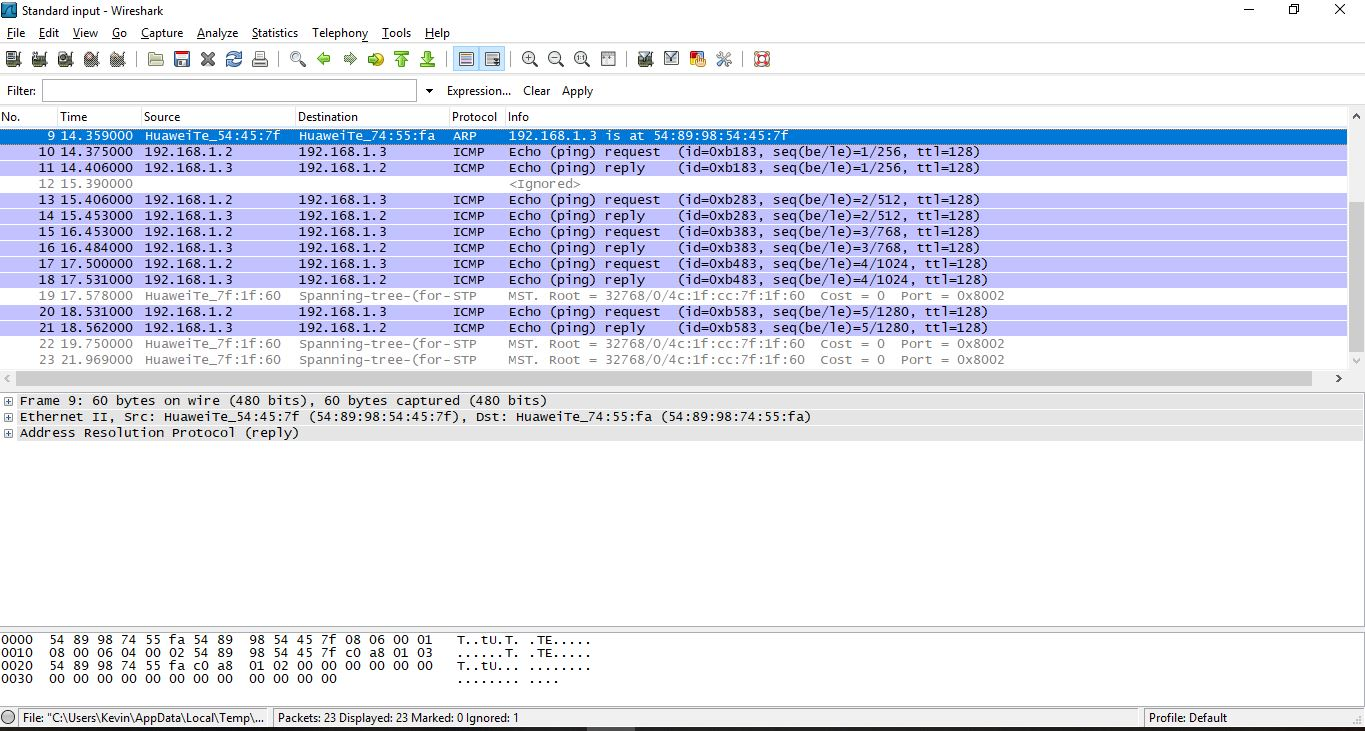
\includegraphics[scale=0.2]{13.JPG} 
\end{figure}
\end{center}
%%%%%%%%%%%
\section{Ejercicios}
Realizar una red LAN Inalámbrica (WLAN) en Packet Tracer y en eNSP, la red debe ser la misma de modo de que se cumplan las siguientes condiciones:
\begin{enumerate}
	\item El número de dispositivos conectados a la red debe ser igual al último número de su código. Teniendo en cuenta que si su último número está en el rango de 0 a 4 le sume 5 dispositivos a la red.
	\item Definir una seguridad WPA2(comunmente vista dispositivos actuales como WPA2/PSK), y la contraseña definida debe ser el número de su código
\end{enumerate}
Enviar la simulación a los correos \url(jujjaramillogr@unal.edu.co) y \url(klcerpac@unal.edu.co), a ambos correos. Plazo hasta el viernes 08 de marzo de 2019.


\begin{thebibliography}{3}
	\bibitem{pt_wiki} \textbf{Packet Tracer}, Wikipedia La Enciclopedia Libre, \url{es.wikipedia.org/wiki/Packet_Tracer}
\end{thebibliography}

\end{document}
%%\textit{End Devices}